\hspace{4mm} Dans ce chapitre, nous abordons la phase d’analyse et spécification des besoins. Ainsi, nous présentons les besoins fonctionnels et non fonctionnels de notre système. Nous décrivons ensuite les principaux cas d'utilisation par le language UML qui représente un moyen simple et facile à comprendre.
\section{	Besoins fonctionnels }
\hspace{4mm} Cette partie décrit les exigences que le système doit satisfaire d’une façon informelle. 
\par Les fonctionnalités qu’on propose de fournir dans notre plateforme sont les suivantes:
\par \textbf{Gestion de projet}
\begin{itemize}
    \item	Chaque projet a un responsable qui peut être un chef de projet ou un membre de l’équipe.
    \item 	Le responsable peut réassigner le projet à n’importe quel utilisateur.
    \item Le responsable de projet a toutes les autorisations pour gérer le projet (modification, ajout ou affectation des tâches….).
    \item Un projet peut avoir plusieurs personnes qui travaillent dessus.
    \item Le chef de projet peut avoir plusieurs projets. 
    \item 	Tous les membres de l’entreprise peuvent voir les états des projets grâce aux diagrammes de GANTT.
    \item 	L'invité (qui va être introduit ci-dessous) peut consulter des cartes et des diagrammes de GANTT.
    \item L'invité peut recevoir des notifications de réunions.
\end{itemize}
\par \textbf{Gestion des tâches}
\begin{itemize}
    \item 	Chaque tâche a un responsable qui peut être le chef de projet, le chef d'équipe ou un membre de l’équipe.
    \item 	Le responsable d’une tâche a les autorisations de modification sur la tâche.
    \item 	Une tâche fait partie d’un seul projet.
    \item 	Chaque membre d’un projet peut participer à plusieurs tâches.
    \item Chaque membre d’un projet peut commenter une tâche comme il peut commenter le projet.
\end{itemize}
\par\textbf{Emploi du temps}
\begin{itemize}
    \item 	Chaque membre doit entrer toutes ses heures de travail.
    \item 	Chaque heure entrée correspond à une tâche du projet.
    \item L’entrée des heures de travail se fait le jour même où le jour suivant.
    \item La saisie des vacances, maladies et autres congés se fait dans la plateforme.
    \item 	Le chef d'équipe doit valider les emplois du temps.
    \item 	Le chef d'équipe peut saisir les emplois du temps pour les membres de son équipe.
    \item 	Le chef d'équipe peut saisir les prévisions de congés d'un autre membre de son équipe.
\end{itemize}
\par\textbf{Gestion des ressources humaines}
\begin{itemize}
    \item 	L’administrateur peut ajouter, modifier et supprimer des membres d’une équipe de travail.
    \item 	L’administrateur peut ajouter et modifier des équipes de travail.
    \item Le chef de projet peut éditer les autorisations d'un membre d’une équipe.
\end{itemize}
\par \textbf{Gestion de communication}
\begin{itemize}
    \item 	Le membre d’un projet peut organiser des réunions s'il a l’autorisation de le faire.
    \item 	L’invité peut participer à des réunions.
    \item Le membre d’un projet peut envoyer/corriger des comptes rendus suite à une réunion s’il y a participé.
    \item 	Le membre d’un projet peut recevoir des comptes rendus.
\end{itemize}
\section{	Besoins non Fonctionnels}
\hspace{4mm}Ce sont des exigences qui ne concernent pas spécifiquement le comportement de la plateforme mais plutôt qui identifient des contraintes internes et externes de la plateforme. 
\par Les principaux besoins non fonctionnels de notre plateforme se résument dans les points suivants :
\begin{itemize}
    \item \textbf{	Ergonomie : }notre application doit offrir une interface conviviale et ergonomique exploitable par l'utilisateur en envisageant les interactions via le navigateur web.
    \item \textbf{	Compatibilité : }l’un des points les plus importants lors du développement d’une application sur un environnement web ou mobile, c’est d’assurer sa compatibilité avec toutes les versions du système ; n’importe quels version et type de navigateur.
    \item \textbf{	La sécurité de l’accès aux informations critiques : }nous devons prendre en considération la confidentialité des données des utilisateurs à travers Spring security et JWT surtout au niveau de l’authentification.
    \item \textbf{	Maintenabilité : }Pendant la phase de maintenance, le code de notre application doit être facile à lire et à comprendre. À cette fin, nous avons décidé de bien commenter le code pour le rendre facile à comprendre et d’utiliser des noms significatifs pour les classes et les variables.
    \item \textbf{	Les contraintes de disponibilité : }l’application doit être disponible pour être utilisée par n’importe quel utilisateur.
\end{itemize}
\section{	Diagrammes de cas d'utilisation}
\hspace{4mm}Dans ce qui suit, nous présentons un formalisme semi formel de spécification des besoins de notre système, à l’aide de diagrammes de cas d’utilisation accompagnés par une description textuelle.
\par Cette description permet de clarifier le déroulement de la fonctionnalité et d’identifier les parties redondantes pour en déduire des cas d’utilisation plus précis qui seront utilisés par inclusion, extension ou généralisation.
\par Dans sa forme textuelle un cas d’utilisation est une collection de scénarios de succès et d’échecs qui décrivent la façon dont un acteur particulier utilise le système pour atteindre un objectif.
\par Les termes suivants sont utilisés pour chaque cas d’utilisation :
\begin{itemize}
    \item \textbf{ Précondition : }définit ce qui doit être vrai en amont afin que le processus puisse démarrer.
    \item \textbf{	Déclencheur : }action qui déclenche le scénario.
    \item \textbf{ Scénario nominal : }scénario qui satisfait l’objectif des acteurs par le chemin le plus direct.
    \item \textbf{	Extensions : }tous les autres scénarios ou branchements possibles aussi bien de succès que d’échec.
\end{itemize}
\subsection{	Identification des acteurs}
\hspace{4mm}Un acteur représente un rôle joué par une entité externe qui interagit directement avec la plateforme mise en place. Il peut consulter et/ou modifier directement l’état du système, en émettant et/ou recevant des messages susceptibtles d’être porteurs de données. \cite{1}
\par Les acteurs suivants ont été identifiés :
\begin{itemize}
    \item 	Invité : qui a des droits de consultation uniquement.
    \item  Membre de la société : qui a des droits restreints sur le projet en question et qui peuvent être définis par le chef de projet.
    \item Chef de projet : qui a des droits sur les projets et les équipes sous sa responsabilité.
    \item	Chef d’équipe : qui est un membre responsable d’une ou de plusieurs équipes.
    \item 	Administrateur : qui est un membre qui s’occupe de l’administration de l’entreprise.
\end{itemize}
\par Il existe des relations d’héritage entre les différents acteurs :
\begin{itemize}
        \item[-] Les invités sont étendus en des membres.
        \item[-] Les membres sont étendus en chefs de projet.
        \item[-] Les chefs de projets sont étendus en chefs d'équipes.
        \item[-] Les chefs d’équipes sont étendus en administrateur, qui a des privilèges supplémentaires comme on peut le voir sur le diagramme "Diagramme de cas d’utilisation Invité " (figure \ref{fig:cas_invi}).
\end{itemize}
\subsection{ Identification des cas d’utilisation}
\hspace{4mm}Les cas d’utilisation représentent un ensemble de séquences d’actions qui sont réalisées par le système et qui produisent un résultat observable intéressant pour un acteur principal. 
\par Dans la collection des cas d’utilisation, sont énumérés tous les processus principaux du système à savoir :
\begin{itemize}
    \item 	Authentification
    \item 	Réception des comptes rendus
    \item 	Participation à des réunions
    \item	Réception des notifications
    \item	Gestion des tâches
    \item	Faire des recherches
    \item	Géstion des les comptes rendus
    \item	Organisation des réunions
    \item	Modification de ses informations
    \item	Saisie de l'emploi du temps
    \item	Saisie des commentaires
    \item	Saisie des prévisions de congés
    \item	Gestion de projet
    \item	Assignation des tâches
    \item	Edition des autorisations pour un autre membre
    \item	Edition des abonnées
    \item	Suivi de projet
    \item	Validation des emplois du temps
    \item	Saisie des emplois du temps de son équipe
    \item	Saisie des prévisions de congés pour son équipe
    \item	Gestion des utilisateurs
    \item	Souscription d'une offre
    \item	Paramétrage général
    \item	Gestion des équipes
\end{itemize}\newpage
\subsection{	Diagrammes généraux}
\hspace{4mm}Dans cette partie, nous présentons les diagrammes des cas d’utilisation détaills ainsi que leurs descriptions textuelles.
\par	\textbf{L’invité :}c’est une personne qui est invitée par email à la plateforme pour recevoir des notifications concernant un projet, participer à une réunion et recevoir des comptes rendus ou des cartes et des diagrammes.

\begin{figure}[h]
    \centering
    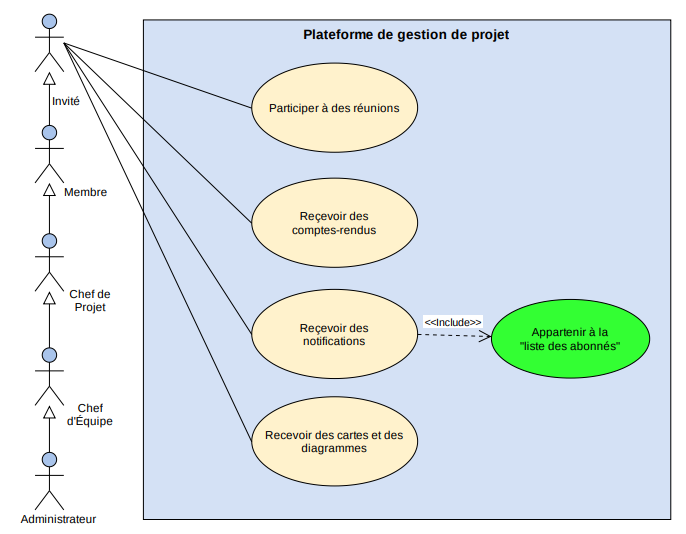
\includegraphics[scale=0.7]{figures/a4.png}
    \caption{Diagramme de cas d’utilisation pour l’invité}
    \label{fig:cas_invi}
\end{figure}
\newpage\par \textbf{	Membre :} cet acteur est un membre ajouté par l'administrateur qui a des missions à faire comme on peut le voir sur le diagramme (Figure \ref{fig:cas_memb}).

\begin{figure}[h]
    \centering
    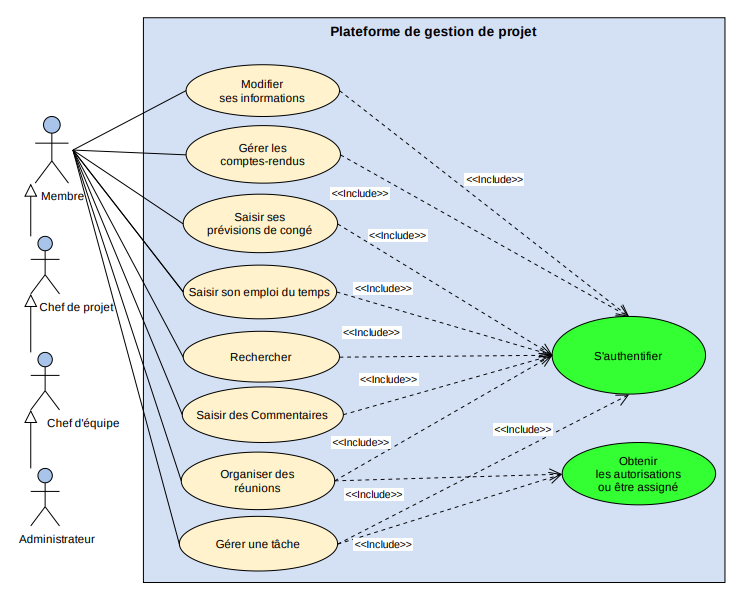
\includegraphics[scale=0.7]{figures/a9.png}
    \caption{Diagramme de cas d’utilisation pour un membre}
    \label{fig:cas_memb}
\end{figure}\newpage
\par \textbf{Chef de projet :} cet acteur est un chef de projet ajouté par l'administrateur qui a des missions à faire comme on peut le voir sur le diagramme (Figure \ref{fig:cas_chefp}).
\begin{figure}[h]
    \centering
    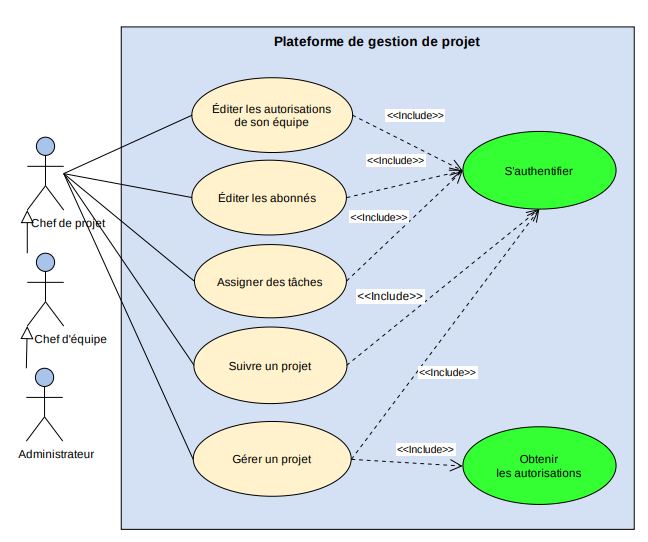
\includegraphics[scale=0.7]{figures/a1.png}
    \caption{Diagramme de cas d’utilisation pour le chef de projet}
    \label{fig:cas_chefp}
\end{figure}
\newpage
\par \textbf{	Chef d’équipe :} cet acteur est un chef d’équipe ajouté par l'administrateur qui a des missions à faire comme on peut le voir sur le diagramme (Figure \ref{fig:cas_chefe}).
\begin{figure}[h]
    \centering
    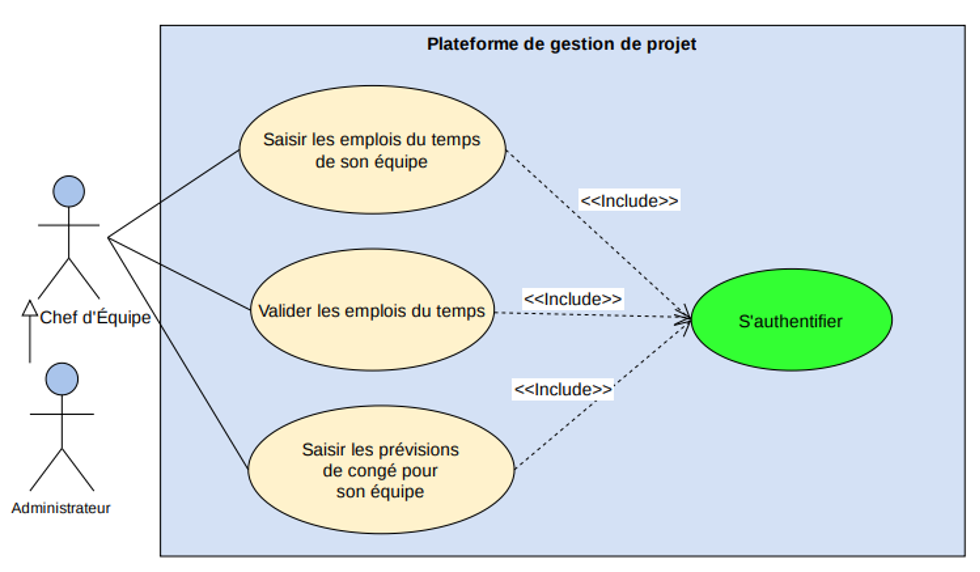
\includegraphics[scale=0.8]{figures/anis7.png}
    \caption{Diagramme de cas d’utilisation pour le chef d’équipe}
    \label{fig:cas_chefe}
\end{figure}

\par \textbf{ Administrateur :} cet acteur est un administrateur qui a des missions à faire comme on peut le voir sur le diagramme (Figure \ref{fig:cas_admin}).
\begin{figure}[h]
    \centering
    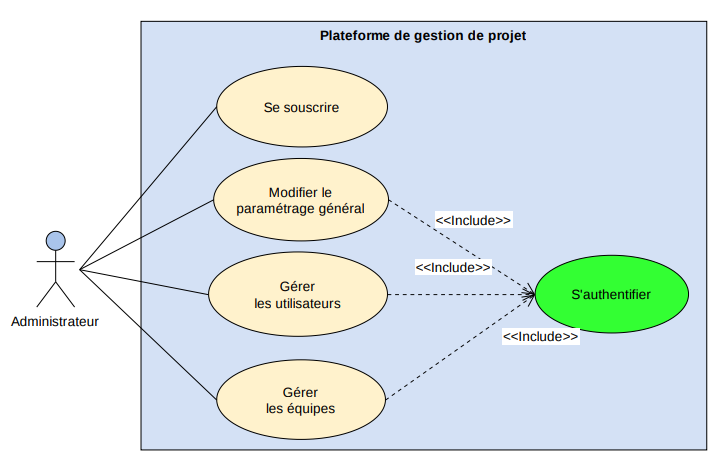
\includegraphics[scale=0.53]{figures/3333anis1.png}
    \caption{Diagramme de cas d’utilisation pour l’administrateur}
    \label{fig:cas_admin}
\end{figure}\newpage
\subsubsection{	Authentification}
\hspace{4mm}L’authentification est la condition préalable nécessaire à tous les autres processus décrits dans les diagrammes des cas d’utilisation. Elle doit être assurée pour permettre aux acteurs d’exécuter leurs propres cas d’utilisation. Le tableau ci-dessous décrit le processus d'authentification.
\begin{center}
\begin{tabular}{|c|l|}
\hline 
&\textbf { Description }\\\hline 
    Acteur principal & Utilisateur \\\hline 
    Objectif&L’utilisateur s’authentifie dans la plateforme.\\\hline
    Préconditions&Les données personnelles permettant l’authentification existent \\&dans la plateforme.\\\hline 
    Déclencheur&L’utilisateur ouvre la page d’authentification de la plateforme\\\hline 
    &Le système affiche un formulaire de login avec les champs email \\&d’utilisateur et mot de passe.\\
    Scénario nominal&L’utilisateur remplit les valeurs du formulaire et sélectionne \\&" Se connecter " une fois terminé.\\& Le système valide les données.\\
    &Le système permet à l’utilisateur de rentrer dans la plateforme.\\\hline
    &Le login échoue si : \\
    Extensions&le couple de valeurs email d’utilisateur + mot de passe ne se trouvent \\
    &pas dans la plateforme.\\\hline
\end{tabular}
\captionof{table}{Description du processus d’authentification}
\label{desc_auth}
\end{center}\newpage
\subsubsection{	Gestion des utilisateurs}
La figure \ref{fig:cas_gerutil} présente le diagramme de gestion de projet.
\begin{figure}[h]
    \centering
    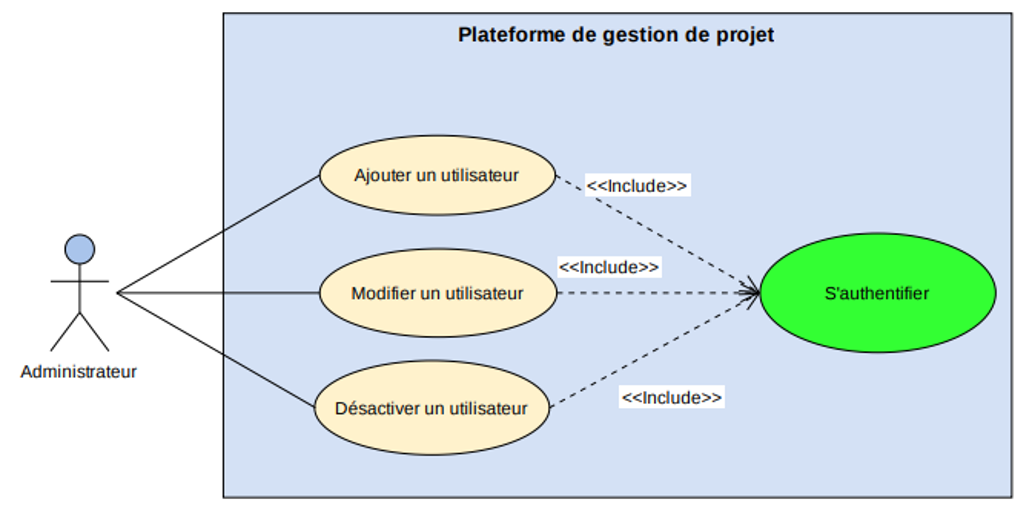
\includegraphics[scale=1]{figures/anis10.png}
    \caption{Diagramme de gestion des utilisateurs par l’administrateur}
    \label{fig:cas_gerutil}
\end{figure}
\par Dans la suite on va détailler les processus de gestion des utilisateurs par l’administrateur aux moyens de tableaux descriptifs.\newpage
\par \textbf{ 	Ajouter un utilisateur}
\par Le tableau suivant présente l’enchainement du cas d’utilisation "Ajouter un utilisateur"
\begin{center}
\begin{tabular}{|c|l|}
\hline 
&\textbf { Description }\\\hline 
    Acteur principal & Administrateur \\\hline 
    Objectif&L’administrateur doit pouvoir ajouter un utilisateur.\\\hline
    Préconditions&Il doit être authentifié.  \\&Il doit être administrateur.\\\hline 
    Déclencheur&L’administrateur choisit " Ajouter un utilisateur "\\\hline 
    &Le système affiche un formulaire d’ajout d’un utilisateur  \\& vide contenant les champs suivants : \\
    &Nom, prénom, email, mot de passe, équipe (liste à \\
    &choix d’équipe), rôle (liste à choix contenant Invité, membre,\\Scénario nominal&chef de projet, chef d’équipe, administrateur),liste des autorisations.\\
    &L’administrateur remplit les valeurs du formulaire \\
    & et sélectionne " enregistrer " une fois terminé.\\
    &Le système valide les données. \\
    &Le système enregistre l’utilisateur.  \\
    &Le système affiche le résultat : succès ou échec. \\\hline
    &L’enregistrement échoue si :  \\
    Extensions&les valeurs minimales ne sont pas remplies.  \\
    &un utilisateur avec ce mail existe déjà.\\\hline
\end{tabular}
\captionof{table}{Description du processus d'ajout d'un utilisateur}
\label{desc_ajout_ut}
\end{center}\newpage
\par \textbf{ 	Modifier un utilisateur}
\par Le tableau suivant présente l’enchainement du cas d’utilisation " Modifier un utilisateur "
\begin{center}
\begin{tabular}{|c|l|}
\hline 
&\textbf { Description }\\\hline 
    Acteur principal & Administrateur \\\hline 
    Objectif&L’administrateur doit pouvoir modifier un utilisateur.\\\hline
    Préconditions&Il doit être authentifié.  \\&Il doit être administrateur.\\\hline 
    Déclencheur&L’administrateur choisit un utilisateur "\\\hline 
    &Le système affiche le formulaire de l'utilisateur choisie   \\&contenant les champs suivants : \\
    &Nom, prénom, email, mot de passe, équipe (liste à \\
    &choix d’équipe), rôle (liste à choix contenant Invité, membre,\\Scénario nominal&chef de projet, chef d’équipe, administrateur).\\
    &L’administrateur remplit les valeurs du formulaire \\
    & et sélectionne " enregistrer " une fois terminé.\\
    &Le système valide les données. \\
    &Le système enregistre les modifications.   \\
    &Le système affiche le résultat : succès ou échec. \\\hline
    &L’enregistrement échoue si :  \\
    Extensions&les valeurs minimales ne sont pas remplies.  \\\hline
\end{tabular}
\captionof{table}{Description du processus de modification d'un utilisateur}
\label{desc_modif_ut}
\end{center}\newpage
\par \textbf{ 	 	Désactiver un utilisateur}
\par Le tableau suivant présente l'enchaînement du cas d'utilisation "désactiver un utilisateur".
\begin{center}
\begin{tabular}{|c|l|}
\hline 
&\textbf { Description }\\\hline 
    Acteur principal & Administrateur \\\hline 
    Objectif&L’administrateur doit pouvoir désactiver les données des utilisateurs.\\\hline
    Préconditions&Il doit être authentifié.  \\&Il doit être administrateur.\\\hline 
    Déclencheur&L’administrateur choisit un utilisateur de la liste des utilisateurs.\\\hline 
    &Le système affiche le formulaire de l’utilisateur choisi.    \\&L’administrateur choisit le bouton Désactiver.  \\
    Scénario nominal&Le système demande confirmation. \\
    &Le système valide la désactivation et l’exécute.  \\
    &Le système affiche le résultat : succès ou échec. \\\hline
    &La désactivation échoue si :   \\
    Extensions&l’utilisateur a fait des saisies des tâches ou des heures   \\
    &dans le système.\\\hline
\end{tabular}
\captionof{table}{Description du processus de désactivation d'un utilisateur}
\label{desc_desact_ut}
\end{center}\newpage
\subsubsection{	Gestion des équipes}
\hspace{4mm}La figure suivante présente le diagramme de gestion des équipes.
\begin{figure}[h]
    \centering
    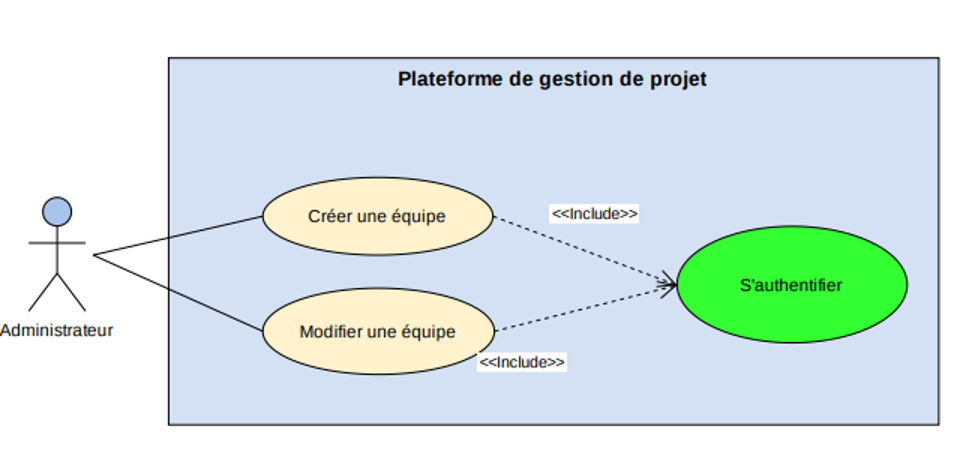
\includegraphics[scale=1]{figures/anis11.png}
    \caption{Diagramme de cas d'utilisation de la gestion des équipes par l’administrateur}
    \label{fig:cas_gereq}
\end{figure}
\par Dans la suite on va détailler les processus de gestion des équipes par l’administrateur aux moyens de tableaux descriptifs.
\newpage
\par \textbf{ 	Créer une équipe}
\par Le tableau suivant présente l'enchaînement du cas d'utilisation "créer une équipe".
\begin{center}
\begin{tabular}{|c|l|}
\hline 
&\textbf { Description }\\\hline 
    Acteur principal & Administrateur \\\hline 
    Objectif&L’administrateur doit pouvoir créer une équipe.\\\hline
    Préconditions&Il doit être authentifié.  \\&Il doit être administrateur.\\\hline 
    Déclencheur&L’administrateur choisit " Ajouter une équipe "\\\hline 
    &Le système affiche un formulaire d’ajout d’une équipe     \\&vide contenant les champs suivants :   \\
    &Nom de l’équipe, nom de projet (liste à choix), chef  \\
    &d’équipe (liste à choix), membres (liste à choix).\\
    &L’administrateur remplit les valeurs du formulaire et \\
    Scénario nominal&et sélectionne " enregistrer " une fois terminé.  \\
    &Le système valide les données. \\
    &Le système enregistre l'équipe. \\
    &Le système affiche le résultat : succès ou échec. \\
    &Le système envoie une notification à tous les utilisateurs \\&qui font partie de cette équipe.\\\hline
    &La désactivation échoue si :   \\
    Extensions&les valeurs minimales ne sont pas remplies.   \\
    &une équipe avec ce nom existe déjà.\\\hline
\end{tabular}
\captionof{table}{Description du processus d'ajout d'une équipe}
\label{desc_ajout_eq}
\end{center}\newpage
\par \textbf{ 	 	Modifier une équipe}
\par Le tableau suivant présente l’enchainement du cas d’utilisation "Modifier une équipe"
\begin{center}
\begin{tabular}{|c|l|}
\hline 
&\textbf { Description }\\\hline 
    Acteur principal & Administrateur \\\hline 
    Objectif&L’administrateur doit pouvoir modifier une équipe.\\\hline
    Préconditions&Il doit être authentifié.  \\&Il doit être administrateur.\\\hline 
    Déclencheur&L’administrateur choisit une équipe de la liste des équipes.\\\hline 
    &Le système affiche le formulaire de l'équipe choisie   \\&contenant les champs suivants :   \\
    &Nom de l’équipe, nom de projet (liste à choix),  \\
    &chef d’équipe (liste à choix), membre (liste à choix).\\
    &L’administrateur change les valeurs du formulaire et  \\
    Scénario nominal& sélectionne "enregistrer" une fois terminé.\\
    &Le système valide les données. \\
    &Le système enregistre les modifications.   \\
    &Le système affiche le résultat : succès ou échec. \\
    &Le système envoie une notification à tous les utilisateurs\\
    &qui font partie de cette équipe\\\hline
    Extensions&La modification échoue si :  \\
    &les valeurs minimales ne sont pas remplies. \\\hline
\end{tabular}
\captionof{table}{Description du processus de modification d'une équipe}
\label{desc_modif_eq}
\end{center}\newpage
\subsubsection{	Gestion de projet}
\par La figure suivante présente le diagramme de cas d’utilisation " Gestion de projet".
\begin{figure}[h]
    \centering
    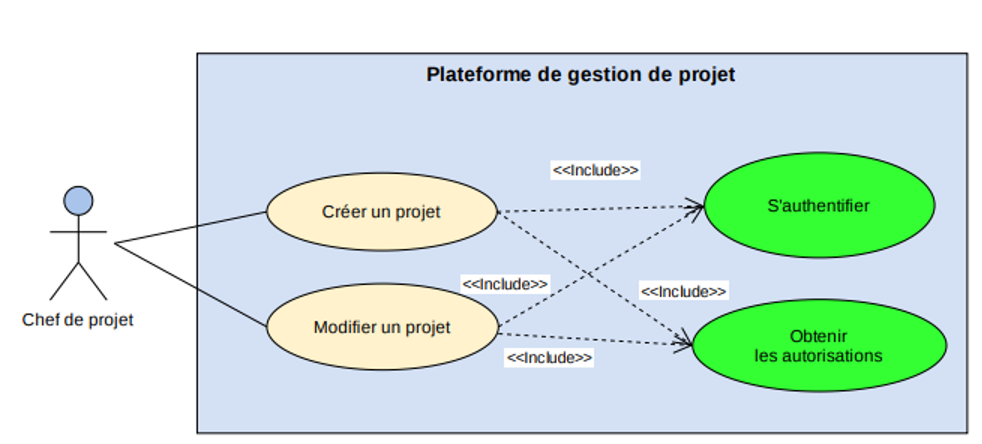
\includegraphics[scale=1]{figures/anis12.png}
    \caption{Diagramme de gestion de projet par le chef de projet}
    \label{fig:cas_gestp_chefp}
\end{figure}
\newpage
\par \textbf{ 	Création d’un projet}
\par Dans la suite on va détailler les processus de gestion de projet par le chef de projet aux moyens de tableaux descriptifs.
\begin{center}
\begin{tabular}{|c|l|}
\hline 
&\textbf { Description }\\\hline 
    Acteur principal & Chef de projet, chef d’équipe, Administrateur \\\hline 
    Objectif&Les acteurs doivent pouvoir créer un projet.\\\hline
    Préconditions&L’acteur doit être authentifié et doit avoir les autorisations.  \\\hline 
    Déclencheur&L’acteur choisit « Création de projet »\\\hline 
    &Le système affiche un formulaire de création de projet    \\&vide contenant les champs suivants :  \\
    &Nom de projet, date début, date fin, chef de projet   \\
    &(liste à choix des membres), description.\\
    Scénario nominal&L’acteur remplit les valeurs du formulaire et sélectionne   \\
    & " enregistrer " une fois terminé. \\
    &Le système valide les données. \\
    &Le système enregistre le projet.   \\
    &Le système affiche le résultat : succès ou échec. \\
    &Le système envoie une notification à tous les utilisateurs\\\hline
    &La modification échoue si :  \\
    Extensions&les valeurs minimales ne sont pas remplies.\\\hline
\end{tabular}
\captionof{table}{Description du processus de création d’un projet}
\label{desc_cree_proj}
\end{center}
\newpage
\par \textbf{ 	 	Modifier un projet}

\begin{center}
\begin{tabular}{|c|l|}
\hline 
&\textbf { Description }\\\hline 
    Acteur principal & Chef de projet, chef d’équipe, Administrateur \\\hline 
    Objectif&Les acteurs doivent pouvoir modifier un projet.\\\hline
    Préconditions&L’acteur doit être authentifié et doit avoir les autorisations.  \\\hline 
    Déclencheur&L’acteur choisit un projet de la liste des projets.\\\hline 
    &Le système affiche le formulaire de projet choisi    \\&contenant les champs suivants :  \\
    &Nom de projet, date début, date fin, chef de projet    \\
    &(liste à choix des membres), description.\\
    Scénario nominal&L’acteur modifier les valeurs du formulaire et sélectionne    \\
    & " enregistrer " une fois terminé. \\
    &Le système valide les données. \\
    &Le système enregistre le projet.   \\
    &Le système affiche le résultat : succès ou échec. \\
    &Le système envoie une notification à tous les utilisateurs\\\hline
    &La modification échoue si :  \\
    Extensions&les valeurs minimales ne sont pas remplies.\\\hline
\end{tabular}
\captionof{table}{Description du processus de modification d'un projet }
\label{desc_modif_proj}
\end{center}\newpage
\subsubsection{	Suivi de projet}
\hspace{4mm}La figure suivante présente le diagramme de cas d'utilisation " Suivi de projet".
\begin{figure}[h]
    \centering
    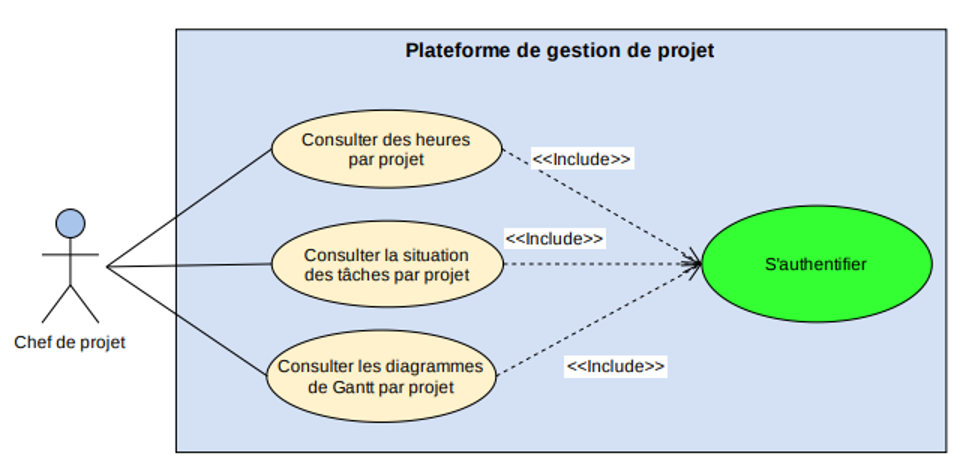
\includegraphics[scale=0.8]{figures/anis13.png}
    \caption{Diagramme de cas d'utilisation de suivi de projet par le chef de projet}
    \label{fig:cas_gestp_chefp}
\end{figure}
\par Dans la suite nous allons détailler les processus des differents cas d'utilisation qui correspondent au suivi de projet.
\par \textbf{  	Consultation des heures par projet	}
\par Ce service permet à certains acteurs de connaitre le nombre d'heures investies dans chaque projet.
\begin{center}
\begin{tabular}{|c|l|}
\hline 
&\textbf { Description }\\\hline 
    Acteur principal & Chef de projet, chef d’équipe, Administrateur \\\hline 
    Objectif&Les acteurs doivent pouvoir consulter les heures d’un projet.\\\hline
    Préconditions&L’acteur doit être authentifié.  \\\hline 
    Déclencheur&L’acteur choisit " Heures par projet "\\\hline 
    &Le système affiche un formulaire de recherche avec tous les projets.   \\
    &L’acteur remplit les valeurs du formulaire et sélectionne    \\
    Scénario nominal&" recherche " une fois terminé. \\
    &Le système effectue la recherche.    \\
    & Le système retourne les données recherchées sous forme de tableau  \\
    &dont toutes les colonnes peuvent être triées et filtrées.  \\\hline
    Extensions&                    - \\\hline
\end{tabular}
\captionof{table}{Description du processus de consultation des heures par projet}
\label{desc_cree_proj}
\end{center}
\newpage
\par \textbf{  	 	Consultation du diagramme de Gantt par projet	}
\par Le tableau suivant présente l’enchainement du cas d’utilisation " Consultation du diagramme de Gantt par projet "
\begin{center}
\begin{tabular}{|c|l|}
\hline 
&\textbf { Description }\\\hline 
    Acteur principal & Chef de projet, chef d’équipe, Administrateur \\\hline 
    Objectif&Les acteurs doivent pouvoir consulter le diagramme de Gantt par projet.\\\hline
    Préconditions&L’acteur doit être authentifié.  \\\hline 
    Déclencheur&L’acteur choisit "Consultation du diagramme de Gantt par projet"\\\hline 
    &Le système affiche un formulaire de recherche avec tous les projets.    \\
    &L'acteur remplit les valeurs du formulaire et sélectionne   \\
    Scénario nominal&" recherche " une fois terminé. \\
    &Le système effectue la recherche.    \\
    & Le système retourne le diagramme de Gantt qui correspond aux critères.   \\
    &Depuis ce diagramme, l’acteur doit pouvoir accéder aux tâches   \\
    &et les modifier.\\\hline
    Extensions&                    - \\\hline
\end{tabular}
\captionof{table}{Description du processus de consultation du diagramme de Gantt par projet}
\label{desc_diag_gantt}
\end{center}
\newpage
\par \textbf{  	 	 	Consultation de la situation des tâches par projet	}
\par Le tableau suivant présente l’enchainement du cas d’utilisation "Consultation de la situation des tâches par projet".
\begin{center}
\begin{tabular}{|c|l|}
\hline 
&\textbf { Description }\\\hline 
    Acteur principal & Chef de projet, chef d’équipe, Administrateur \\\hline 
    Objectif&Les acteurs doivent pouvoir consulter la situation des tâches par projet.\\\hline
    Préconditions&L’acteur doit être authentifié.  \\\hline 
    Déclencheur&L’acteur choisit "Consultation de la situation des tâche par projet"\\\hline 
    &Le système affiche un formulaire de recherche avec tous les projets     \\
    &et les états des tâches (A faire, En cours, Fait).   \\
    &Le chef de projet remplit les valeurs du formulaire et sélectionne  \\
    Scénario nominal&"recherche" une fois terminé.    \\
    & Le système effectue la recherche.   \\
    &Le système retourne les données recherchées sous forme de   \\
    &tableau dont toutes les colonnes peuvent être triées et filtrées.\\\hline
    Extensions&                    - \\\hline
\end{tabular}
\captionof{table}{Description du processus de consultation de la situation des tâches par projet}
\label{desc_tache_proj}
\end{center}
\newpage
\par \textbf{  	 	 	2.4.3.6	Editer les autorisations pour un autre membre	}
\par Tout acteur de type chef d’équipe, chef de projet ou administrateur, dépendamment de son niveau, peut changer les types d'accès du reste des membres de l'équipe qu'il gère.
\par Le tableau ci-dessous décrit le processus d'édition des autorisations pour un autre membre.
\begin{center}
\begin{tabular}{|c|l|}
\hline 
&\textbf { Description }\\\hline 
    Acteur principal & Chef de projet, chef d’équipe, Administrateur \\\hline 
    Objectif&Les acteurs doivent pouvoir éditer les autorisations pour un autre membre.\\\hline
    Préconditions&L’acteur doit être authentifié.  \\\hline 
    Déclencheur&L’acteur choisit un membre de la liste des membres.\\\hline 
    &Le système affiche le formulaire du membre choisi contenant les champs     \\&suivants :\\
    &Nom, prénom, email, mot de passe, équipe, rôle, liste d’autorisation.   \\
    &L’acteur change les valeurs de la liste d'autorisation et sélectionne   \\
    Scénario nominal&" enregistrer " une fois terminé.   \\
    & Le système valide les données.    \\
    &Le système enregistre les modifications.   \\
    &Le système affiche le résultat : succès ou échec.\\
    &Le système envoie une notification d’information à ce membre.\\\hline
      &La modification échoue si :  \\
    Extensions&les valeurs minimales ne sont pas remplies.\\\hline             
\end{tabular}
\captionof{table}{Description du processus d'edition des autorisations pour un autre membre}
\label{desc_edit_autor}
\end{center}
\newpage
\subsubsection{		Gestion des tâches}
\hspace{4mm}La figure suivante présente le diagramme de cas d'utilisation " Gestion des tâches "
\begin{figure}[h]
    \centering
    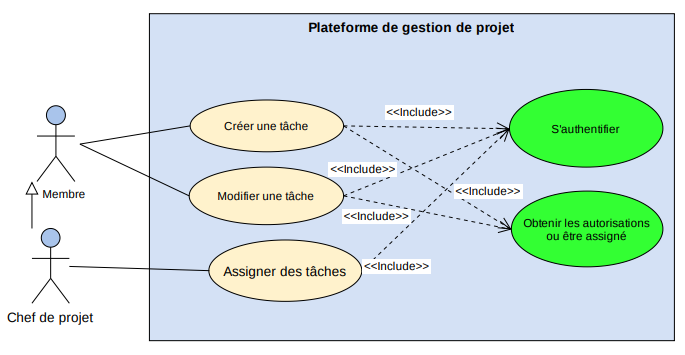
\includegraphics[scale=0.63]{figures/a3.png}
    \caption{Diagramme de cas d'utilisation de gestion des tâches par un membre }
    \label{fig:cas_gerer_tache}
\end{figure}
\par Dans la suite nous allons détailler les processus des différents cas d'utilisations qui correspondent de la gestion des tâches par un membre.
\newpage
\par \textbf{  	 	Création d’une tâche	}
\par Le tableau suivant présente la description du cas d'utilisation de création d'une tâche.
\begin{center}
\begin{tabular}{|c|l|}
\hline 
&\textbf { Description }\\\hline 
    Acteur principal & Chef de projet, chef d’équipe, Administrateur \\\hline 
    Objectif&Les acteurs doivent pouvoir créer une tâche.\\\hline
    Préconditions&L’acteur doit être authentifié et doit avoir les autorisations.  \\\hline 
    Déclencheur&L’acteur choisit " Nouvelle tâche "\\\hline 
    &Le système affiche un formulaire de nouvelle activité vide avec     \\
    &les champs suivants :    \\
    &Sujet, description, date début, date de fin, responsable (liste  \\
    Scénario nominal&à choix des membres), projet (liste à choix des projets).    \\
    & L’acteur remplit le formulaire.  \\
    &Le système valide les données. \\&Le système enregistre la tâche. \\&Le système affiche le résultat : succès ou échec.  \\\hline
    Extensions&La tâche ne peut pas être ajoutée si : \\&les valeurs minimales ne sont pas remplies.\\\hline
\end{tabular}
\captionof{table}{Description du processus de création d’une tâche}
\label{desc_cree_tache}
\end{center}
\newpage
\par \textbf{  	 	 	Assignation et modification des tâches	}
\par Le tableau suivant présente la description du cas d'utilisation de l’assignation et modification des tâches.
\begin{center}
\begin{tabular}{|c|l|}
\hline 
&\textbf { Description }\\\hline 
    Acteur principal & Chef de projet, chef d’équipe, Administrateur \\\hline 
    Objectif&Les acteurs doivent pouvoir assigner les tâches.\\\hline
    Préconditions&L’acteur doit être authentifié et doit avoir les autorisations.  \\\hline 
    Déclencheur&L’acteur choisit "Rechercher une tâche"\\\hline 
    &Le système affiche les paramètres de recherche suivants :      \\
    &Projet, utilisateur, état de l’activité (A Faire, En cours, Fait, Tout).   \\
    &L’acteur choisit ses paramètres et lance la recherche  \\
    Scénario nominal&Le système génère une " Vue " avec toutes les tâches     \\
    & correspondant à la recherche.   \\&L’acteur choisit la tâche qui l’intéresse et l’assigne à un membre.\\
    &Le système valide les données. \\&Le système enregistre la tâche. \\&Le système envoie une notification au membre assigné.\\&Le système affiche le résultat : succès ou échec.  \\\hline
    Extensions&   -\\\hline
\end{tabular}
\captionof{table}{Description du processus d'assignation et modification des tâches}
\label{desc_modif_tache}
\end{center}
\newpage
\par \textbf{  	 	Organiser des réunions	}
\par Le tableau suivant présente l’enchainement du cas d’utilisation "Organiser des réunions".
\begin{center}
\begin{tabular}{|c|l|}
\hline 
&\textbf { Description }\\\hline 
    Acteur principal & Chef de projet, chef d’équipe, Administrateur \\\hline 
    Objectif&Les acteurs doivent pouvoir organiser une réunion.\\\hline
    Préconditions&L’acteur doit être authentifié.  \\\hline 
    Déclencheur&L’acteur choisit " Nouvelle réunion "\\\hline 
    &Le système affiche un formulaire de nouvelle réunion vide       \\
    &avec les champs suivants :    \\
    &Organisateur, Objet, description, horaire/date, participants   \\
    Scénario nominal&(liste à choix des membres), emplacement.     \\
    & L’acteur remplit le formulaire.    \\
    &Le système valide les données. \\&Le système enregistre la réunion.  \\&Le système affiche le résultat : succès ou échec.  \\\hline
    Extensions&  La réunion ne peut pas être ajoutée si : \\&les valeurs minimales ne sont pas remplies.\\\hline
\end{tabular}
\captionof{table}{Description du processus d'organisation des réunions}
\label{desc_org_reunion}
\end{center}
\newpage
\par \textbf{  	Saisie emploi du temps	}
\par Le tableau suivant présente l’enchainement du cas d’utilisation "Saisie emploi du temps".
\begin{center}
\begin{tabular}{|c|l|}
\hline 
&\textbf { Description }\\\hline 
    Acteur principal & Chef de projet, chef d’équipe, Administrateur \\\hline 
    Objectif&Les acteurs doivent pouvoir saisir leurs emplois du temps.\\\hline
    Préconditions&L’acteur doit être authentifié.  \\\hline 
    Déclencheur&L’acteur choisit "Saisie emploi du temps"\\\hline 
    &L’utilisateur choisit le projet, la tâche, la date, la description       \\
    &et le nombre d’heures.     \\
    Scénario nominal&L’utilisateur soumet les valeurs au serveur.   \\
    &Le serveur valide les données, les enregistre et retourne le résultat    \\
    & à l’utilisateur : succès ou échec.   \\
    \hline
    Extensions&  L'emploi du temps ne peut pas être ajoutée si : \\&les valeurs minimales ne sont pas remplies.\\\hline
\end{tabular}
\captionof{table}{Description du processus de saisie de l'emploi du temps}
\label{desc_emp_temps}
\end{center}

\subsubsection{		Gestion des comptes rendus}
\hspace{4mm}La figure suivante présente le diagramme de cas d'utilisation "Gérer les comptes rendus"
\begin{figure}[h]
    \centering
    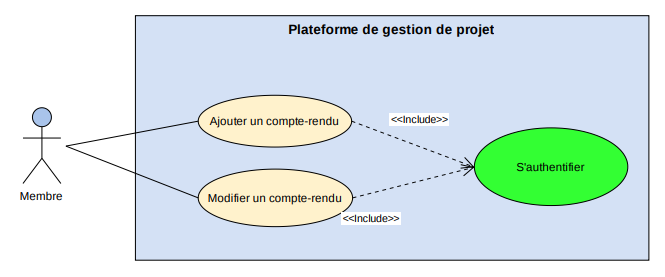
\includegraphics[scale=0.65]{figures/a2.png}
    \caption{Diagramme de cas d'utilisation de gestion des comptes rendus par un membre }
    \label{fig:cas_gerer_cmpterendu}
\end{figure}
\par Dans la suite nous allons détailler les processus des différents cas d'utilisations qui correspondent à la gestion des comptes rendus.
\par \textbf{  	 	 	 	Ajouter un compte-rendu	}
\par Le tableau suivant présente l’enchainement du cas d’utilisation "Ajouter un compte rendu".
\begin{center}
\begin{tabular}{|c|l|}
\hline 
&\textbf { Description }\\\hline 
    Acteur principal & Chef de projet, chef d’équipe, Administrateur \\\hline 
    Objectif&Les acteurs doivent pouvoir ajouter un compte-rendu.\\\hline
    Préconditions&L’acteur doit être authentifié.  \\\hline 
    Déclencheur&L’acteur choisit " Ajouter un compte-rendu "\\\hline
    &Le système affiche un formulaire de nouveau compte-rendu   \\
    &vide avec les champs suivants :    \\
    &Réunion (liste à choix des réunions), description (elle regroupe  \\
    &les points déjà mentionnés dans l’invitation à la réunion avec la      \\
    Scénario nominal& possibilité d’ajouter des points supplémentaires), participants    \\&(liste à choix des utilisateurs).\\&L’acteur remplit le formulaire. \\
    &Le système valide les données. \\&Le système enregistre le compte-rendu.  \\&Le système affiche le résultat : succès ou échec.  \\&Le système envoie une notification aux utilisateurs participants.\\\hline
    Extensions&   L’enregistrement échoue si :\\&les valeurs minimales ne sont pas remplies.\\\hline
\end{tabular}
\captionof{table}{Description du processus de gestion des comptes rendus}
\label{desc_gerer_cmpterendu}
\end{center}
\newpage
\par \textbf{  	Modifier un compte-rendu	}
\par Le tableau suivant présente l’enchainement du cas d’utilisation "Modifier un compte rendu".
\begin{center}
\begin{tabular}{|c|l|}
\hline 
&\textbf { Description }\\\hline 
    Acteur principal & Chef de projet, chef d’équipe, Administrateur \\\hline 
    Objectif&Les acteurs doivent pouvoir modifier un compte-rendu.\\\hline
    Préconditions&L’acteur doit être authentifié.  \\\hline 
    Déclencheur&L’acteur choisit un compte-rendu de la liste des comptes rendus.\\\hline
    &Le système affiche le formulaire du compte-rendu choisi    \\
    &contenant les champs suivants :    \\
    &Réunion (liste à choix des réunions), description (elle regroupe  \\
    &les points déjà mentionnés dans l’invitation à la réunion avec la      \\
    Scénario nominal& possibilité d’ajouter des points supplémentaires), participants    \\&(liste à choix des utilisateurs).\\&L’acteur modifie le formulaire. \\
    &Le système valide les données. \\&Le système enregistre les modifications apportées au compte-rendu.  \\&Le système affiche le résultat : succès ou échec.  \\&Le système envoie une notification aux utilisateurs participants.\\\hline
    Extensions&   L’enregistrement échoue si :\\&les valeurs minimales ne sont pas remplies.\\\hline
\end{tabular}
\captionof{table}{Description du processus de modification des comptes rendus}
\label{desc_modif_cmpterendu}
\end{center}
\newpage
\subsubsection{	Saisie de prévision de congé	}
\par Le tableau suivant présente l’enchainement du cas d’utilisation "Saisie prévision de congé".
\begin{center}
\begin{tabular}{|c|l|}
\hline 
&\textbf { Description }\\\hline 
    Acteur principal & Chef de projet, chef d’équipe, Administrateur \\\hline 
    Objectif&Les acteurs doivent pouvoir saisir leurs prévisions de congé.\\\hline
    Préconditions&L’acteur doit être authentifié.  \\\hline 
    Déclencheur&L’acteur choisit "Saisie prévision de congé"\\\hline
    &Le système affiche un formulaire de nouvelle prévision de congé\\
    &vide avec les champs suivants :    \\
    &Date début, date fin.   \\
   &L’acteur remplit le formulaire.  \\
    &Le système valide les données. \\&Le système enregistre la prévision de congé. \\&Le système affiche le résultat : succès ou échec.  \\&Le système envoie une notification à l’administrateur.\\\hline
    Extensions&   L’enregistrement échoue si :\\&les valeurs minimales ne sont pas remplies.\\\hline
\end{tabular}
\captionof{table}{Description du processus de saisie de prévision de congé}
\label{desc_saisie_conge}
\end{center}


\section*{Conclusion}
\hspace{4mm} Ce chapitre nous a permis de présenter les besoins fonctionnels de l’utilisateur et de définir les besoins non fonctionnels à prendre en considération afin de le satisfaire les utilisateurs et de détailler les cas d’utilisation de notre plateforme. La spécification des besoins étant établie, le chapitre suivant présentera une conception claire de l’architecture de la
plateforme proposée.  